\let\negmedspace\undefined
\let\negthickspace\undefined
\documentclass[journal]{IEEEtran}
\usepackage[a5paper, margin=10mm, onecolumn]{geometry}
%\usepackage{lmodern} % Ensure lmodern is loaded for pdflatex
\usepackage{tfrupee} % Include tfrupee package

\setlength{\headheight}{1cm} % Set the height of the header box
\setlength{\headsep}{0mm}     % Set the distance between the header box and the top of the text

\usepackage{gvv-book}
\usepackage{gvv}
\usepackage{cite}
\usepackage{amsmath,amssymb,amsfonts,amsthm}
\usepackage{algorithmic}
\usepackage{graphicx}
\usepackage{textcomp}
\usepackage{xcolor}
\usepackage{txfonts}
\usepackage{listings}
\usepackage{enumitem}
\usepackage{mathtools}
\usepackage{gensymb}
\usepackage{comment}
\usepackage[breaklinks=true]{hyperref}
\usepackage{tkz-euclide} 
\usepackage{listings}
% \usepackage{gvv}                                        
\def\inputGnumericTable{}                                 
\usepackage[latin1]{inputenc}                                
\usepackage{color}                                            
\usepackage{array}                                            
\usepackage{longtable}                                       
\usepackage{calc}                                             
\usepackage{multirow}                                         
\usepackage{hhline}                                           
\usepackage{ifthen}                                           
\usepackage{lscape}
\numberwithin{equation}{enumi}
\begin{document}

\bibliographystyle{IEEEtran}


\title{1-1.2-21}
\author{EE24BTECH11062 - Vuddanti Homa Harshitha
}
% \maketitle
% \newpage
% \bigskip
{\let\newpage\relax\maketitle}

\renewcommand{\thefigure}{\theenumi}
\renewcommand{\thetable}{\theenumi}
\setlength{\intextsep}{10pt} % Space between text and floats

\renewcommand{\thetable}{\theenumi}


\textbf{Question}:\\
Represent graphically a displacement of $40km, 30\degree$  west of south.
\\
\textbf{Solution: }
\begin{table}[h!]    
  \centering
  \begin{tabular}[12pt]{ |c| c|}
    \hline
    \textbf{Variable} & \textbf{Description}\\ 
    \hline
    $a$ & $x$-coordinate of point B\\
    \hline 
    $b$ & $y$-coordinate of point C\\
    \hline
    \end{tabular}


  \caption*{1-1.2-21-Table-1 : Variables Used}
\end{table}

The position vector can be represented as :
\begin{align}
\myvec{x\\y} =\myvec{R\cos\theta\\
 R\sin\theta}\label{1-1.2-21-1}
\end{align}
Given,
\begin{align}
R =40 km\label{1-1.2-21-2}\\
\theta = 240\degree=\frac{4\pi}{3}\label{1-1.2-21-3}
\end{align}
From  equations \eqref{1-1.2-21-1} and \eqref{1-1.2-21-2}, the horizontal and vertical components are:
\begin{align}
\myvec{x \\ y}=\myvec{40\cos\brak{\frac{4\pi}{3}}\\
40\sin\brak{\frac{4\pi}{3}}\\}\\
 \implies
 \myvec{x\\y}=\myvec{-\frac{40}{2}\\-\frac{40\sqrt{3}}{2}}\\
 \implies
 \myvec{x\\y}=\myvec{-20\\-20\sqrt{3}}
\end{align}
 This can be represented graphically as below:
\begin{figure}[h!]
   \centering
   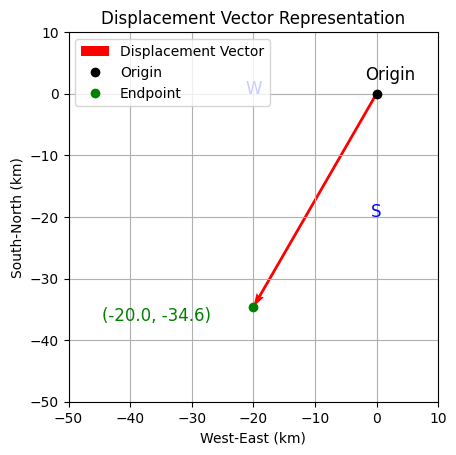
\includegraphics[width=0.5\columnwidth]{figs/fig.png}
   \caption*{1-1.2-21-Figure-1: Graphical representation of the displacement vector}
   \label{1-1.2-21-Figure-1}
\end{figure}
\end{document}  



